% Sovereign Integrity Protocol License v1.1; see the repository LICENSE.
\documentclass[11pt]{article}
\usepackage[T1]{fontenc}
\usepackage[margin=1in]{geometry}
\usepackage{amsmath,amssymb,amsthm,booktabs,graphicx}
\usepackage[expansion=false]{microtype}
\usepackage[hidelinks]{hyperref}
\newtheorem{proposition}{Proposition}
\newcommand{\Tr}{\operatorname{Tr}}
\title{Condensate Binding, Charge Protection,\\and the Boundary of Particle Identification}
\author{Brad Wallace\\\small Independent Researcher}
\date{24 September 2026}
% Publication typography: portable paths, bounded tables, paragraph flexibility.
\usepackage{xurl,adjustbox}
\setlength{\emergencystretch}{3em}
\begin{document}
\maketitle
\begin{abstract}
We separate a tested classical binding mechanism from the identification of
an elementary particle in the ACS condensate program. A specified coupled
real--complex scalar model admits a qualified localized rotating solution
with total energy below its free charged-wave threshold. Independent
discretizations, tail behavior and energy identities support that conditional
result. Explicit charge breaking produces leakage, while weak gauging retains
some scalar--electric solutions but exposes omitted charged vector carriers.
We then test proposed microscopic identifications involving framing,
capacitance, Klein-cover maps, surface projection kernels, internal color
states and Palatini torsion. Exact counterexamples invalidate several
claimed implications while retaining the valid metric, representation and
binding calculations. The result is a reproducible account of what the
reviewed equations establish and which additional dynamical, normalization
and quantum-state inputs are required for a physical mass or lifetime.
\end{abstract}

\section{Introduction}
A localized classical field, a conserved charge and an experimentally
identified particle are distinct requirements. The aim here is to follow the
ACS condensate proposal through those requirements without replacing a
missing derivation by a fitted value or a change of terminology.
The tested binding mechanism belongs to the Friedberg--Lee--Sirlin class,
with a positive complex-field quartic added~\cite{Heeck}. Its numerical
qualification is useful even though its coefficients and physical units
have not been selected by the microscopic proposal.

We first state the reduced model and its controls. We then include an
existing gauge generator and its additional carriers. Finally, we test the
geometric and action-level claims proposed to supply the missing physical
identification. Exact algebraic obstructions are distinguished throughout
from finite numerical observations and untested alternatives.

\section{A specified self-binding model}
Let $\chi$ be real and $q$ complex. In the chosen dimensionless units,
\begin{align}
 E={}&\int_{\mathbb R^3}\left[
 \frac{|q_t|^2+|\nabla q|^2+\chi_t^2+|\nabla\chi|^2}{2}
 +U(\chi,q)\right]d^3x,\\
 U={}&\frac{(\chi^2-1)^2}{4}+\frac{\chi^2|q|^2}{2}
 +\frac b4|q|^4,\qquad
 Q=\int\operatorname{Im}(\bar q q_t)\,d^3x.
\end{align}
The vacuum is $(\chi,q)=(1,0)$ and the exterior charged-wave mass is one.
For $q=f(r)e^{i\omega t}$ and
$I=4\pi\int r^2f^2dr$, the fixed-charge energy is
\begin{equation}
 E_Q=G+V+\frac{Q^2}{2I},\qquad Q=\omega I.
\end{equation}
Here $G$ includes both field gradients. The condensate depletes where the
charged field is large and creates its interior well dynamically; it is not
a prescribed external barrier or a time-dependent energy source.

The inequality $E<|Q|$ prevents complete dispersal into the free charged
waves of this model at fixed charge. It does not exclude all fission
partitions, nonlinear disturbances or quantum decay channels.
An exact control follows by restoring positive coefficients:
\begin{align}
 U-\frac{g^2v^2f^2}{2}
 ={}&\frac{\lambda_\chi}{4}
 \left[(\chi^2-v^2)+\frac{g^2}{\lambda_\chi}f^2\right]^2
 +\frac14\left(b-\frac{g^4}{\lambda_\chi}\right)f^4.
\end{align}
Thus $b\ge g^4/\lambda_\chi$ implies $E\ge gv|Q|$; the tested
$b=1.2$ control cannot have the claimed binding advantage in our units.

\subsection{Qualified numerical reference}
For the chosen $b=2\sqrt3/27$ and $Q=1000$, an independent radial
boundary-value solve gives
\begin{equation}
 E=838.163096,\qquad\omega=0.754888212,
 \qquad \sqrt{1-\omega^2}=0.655853480.
\end{equation}
The fitted exterior tail exponent is $0.655853649$. The relative virial
residual is $2.99\times10^{-10}$ and the maximum boundary-value RMS
residual is $9.91\times10^{-8}$. Finite-volume refinement from spacing
$0.1$ to $0.05$ changes the energy from $838.131320$ to $838.155154$,
consistent with the expected discretization trend.

The tested amplitude and phase sectors have no negative mode; the dipole
mode converges toward the translation zero mode. Conservative dynamics
and prepared-packet formation tests extend to dimensionless time 80.
These are finite tests in the declared scalar model, not an asymptotic
formation theorem or a full-theory particle lifetime. An initial optimizer
failed its gradient criterion; the failed record and subsequent Newton
qualification are both retained, without relaxing the criterion.

\begin{figure}[ht]
\centering
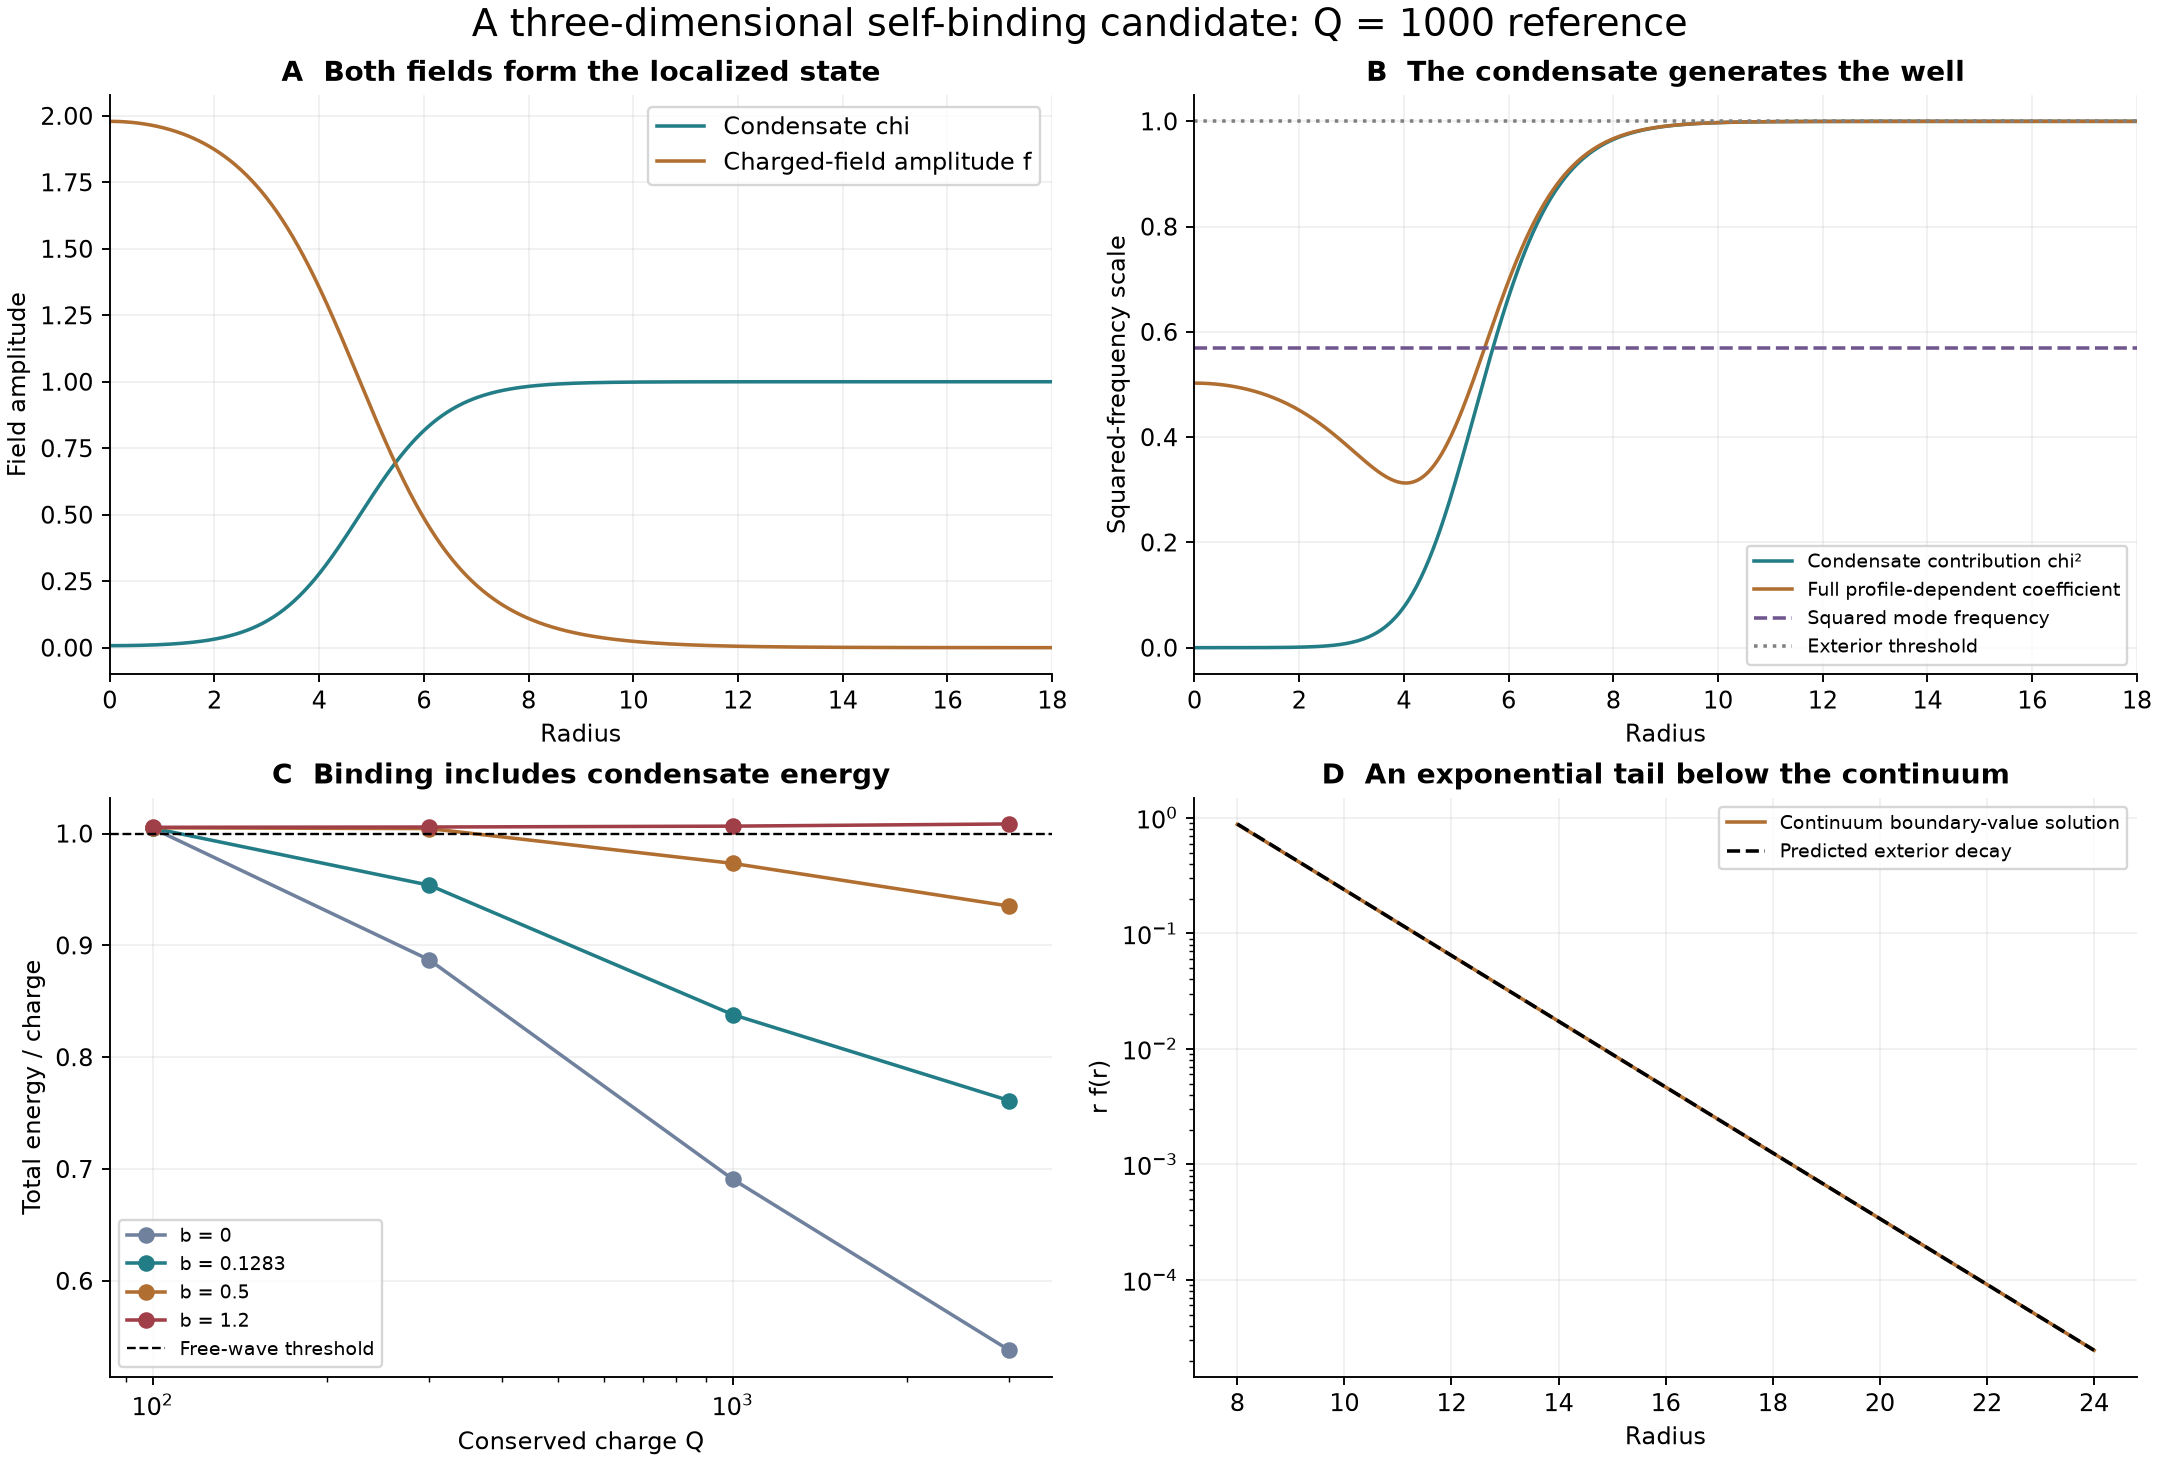
\includegraphics[width=.97\textwidth]{../../docs/condensate_energy/self_binding/binding-evidence.png}
\caption{Conditional scalar binding, with all field energies included.
The coefficient and charge are inputs; the tested profiles do not establish
an elementary-particle identity.}
\end{figure}

\section{Charge breaking and gauge completion}
In the full inherited scalar/Yukawa content, a generic uniform phase of
$\Phi$ is not a symmetry. The allowed holomorphic $\Delta$ quartic breaks
the candidate global $X$ charge; even with that coefficient pair set to zero,
weak mixed anomalies remain. The explicit reduced charge-breaking tests
therefore measure leakage rather than assume an exact global protection.
An independent radiation calculation gives the leading tested power
$P\simeq1.077996267\,\epsilon^2$. A simulated finite charge-loss time is
not an elementary-particle half-life.

For a gauged reduced model use $D_\mu q=(\partial_\mu-ieA_\mu)q$,
$q=f(r)e^{i\omega t}$ and $\Omega=\omega-eA_0$. The equations are
\begin{align}
 \chi''+2\chi'/r&=\chi(\chi^2-1+f^2),\\
 f''+2f'/r&=(\chi^2-\Omega^2)f+bf^3,\\
 \Omega''+2\Omega'/r&=e^2f^2\Omega.
\end{align}
With $A_0(\infty)=0$, the exterior Coulomb contribution beyond radius $R$ is
\begin{equation}
 E_{\rm outside}=\frac{e^2Q^2}{8\pi R},\qquad
 \omega=\Omega(R)+R\Omega'(R).
\end{equation}
Omitting this energy creates a false binding margin. At $Q=1000,e=0.12$,
the total $E/Q=0.96420948$ and $\omega=0.96932000$; $14.323945$ energy
units lie outside the radius-40 domain. Independent finite-volume
minimization, Gauss-law, virial and chemical-potential checks qualify the
selected branch. Solver failures are retained and are not nonexistence proofs.

\subsection{An existing gauge charge brings additional carriers}
The scalar slice
\begin{equation}
 \Phi=\chi I_2/2,\quad D_1=D_2=0,\quad D_3=qE_{44}/\sqrt2,
 \qquad T^{15}=\frac{\operatorname{diag}(1,1,1,-3)}{2\sqrt6}
\end{equation}
has the reduced trace kinetic terms and
$e=\sqrt{3/2}\,g_4$. A selected gauge-invariant potential reproduces
the reduced scalar model. Its rank-one slice also has zero value and
first derivative of the allowed holomorphic invariant, so no illegal
single-component $q^4$ interaction has been silently removed.

However, the exterior $\Phi=I_2/2,\Delta=0$ leaves $SU(4)$ unbroken.
At unit gauge couplings the full 21-generator mass Gram has eighteen
zeros and three eigenvalues $1/2$. Three complex color--lepton vector
pairs are massless and carry $T^{15}$ weight of magnitude $2/3$ of
the selected $\Delta$ component's weight. These classical modes invalidate
using the massive scalar threshold alone as a full-theory stability
certificate. No non-Abelian decay width or quantum confinement conclusion
is inferred from this calculation.

The conventional neutral vacuum used in the companion action paper is a
different background. Its proposed neutral component is electromagnetically
neutral. Its charged partners have calculable spectra, but their masses
and a condensate-to-particle map are not selected. Allowed Yukawa choices
give opposite answers to fermion-emission threshold questions while obeying
the same proposed dimensionless ratio. Additional carrier information is
therefore a physical input, not a plotting choice.

\section{Testing the proposed microscopic identifications}
\subsection{Framing does not determine the magnetic moment}
The torus curve in the earlier note is a $(2,1)$ embedding and an unknot.
The spin-cover class contains a parity bit, whereas a gyromagnetic ratio is
a real-valued dynamical observable. The repository had already withdrawn
the identification of self-linking number with $g$; this amendment applies
that correction consistently to the papers that reused it.

For classical charge and mass moving along the same closed curve with
uniform charge-to-mass ratio, magnetic moment and angular momentum are
proportional to the same oriented vector area. Their conventional ratio
gives $g=1$, independently of winding or framing. Altering charge/current
and mass distributions can change the moment while retaining the curve.
This does not calculate the QED vertex or deny the electron's measured
magnetic moment; it disproves the stated topological inference.

\subsection{Capacitance retains a cutoff and a factor of two}
Let $L=\log(8R/a)+1$ and use the proposed
\begin{equation}
 C=\frac{2\pi\epsilon_0R}{L},\qquad
 q=\frac e2,\qquad R=\frac{\hbar}{2mc}.
\end{equation}
Then $E=q^2/(2C)$ gives
\begin{equation}
 \frac{E}{mc^2}=\frac{\alpha L}{2},\qquad
 E=mc^2\ \Longrightarrow\ \alpha^{-1}=L/2.
\end{equation}
The later archived CPF manuscript instead used $\alpha^{-1}=L$ and
inserted $a/R=8\exp[-(K-1)]$. This produces any desired $L=K$ by
construction. At its chosen $K=137.035999171$, that exponential is
$6.65896\times10^{-59}$; its own self-energy equation requires
$a/R=8\exp[-(2K-1)]\simeq2.03905\times10^{-118}$ to reproduce the
same inverse coupling. Neither cutoff follows from topology. The
companion capacitance computations remain conditional model comparisons.

\subsection{A cover map, a metric and a surface state are separate objects}
For the source's orientation double cover, the deck action on first
homology is $D=\operatorname{diag}(1,-1)$. A lifted quotient
diffeomorphism must commute with its unique nontrivial deck transformation.
The proposed matrix fails this necessary condition:
\begin{equation}
 M=\begin{pmatrix}1&2\\0&1\end{pmatrix},\qquad
 MD-DM=\begin{pmatrix}0&-4\\0&0\end{pmatrix}.
\end{equation}
This does not imply that identity cover homology determines a trivial
mapping class; the earlier topology correction remains in force.
The printed metric, by contrast, respects the glide pullback. Its
determinant $R^2+p^2\cos^2(u/2)/(4\pi^2)$ retains independent radius
and pitch inputs. A valid metric identity does not repair an invalid map.

Integrating a three-dimensional delta kernel over a two-dimensional
surface produces a surface distribution. It does not by itself define
a normalized volume $L^2$ state. A unit-integral transverse Gaussian
of width $\varepsilon$ has squared $L^2$ norm
$1/(2\sqrt\pi\varepsilon)$, diverging as the width tends to zero.
A smearing prescription, state domain and dynamics are required before
the proposed projection can identify a particle.

\subsection{Gauge-invariant statements cannot depend on real versus imaginary labels}
The transformation $\psi\mapsto i\psi$ exchanges real and imaginary
components while preserving $|D\psi|^2$. An imaginary component of a
charged field does not thereby become electromagnetically dark.
Likewise, the supplied Bell state and observables reproduce $2\sqrt2$,
whereas the same settings on a product state give $\sqrt2$. The state
and observables are assumptions, not consequences of a coordinate map.
The manuscript's two-to-three coordinate map has rank two.

The color/music source proposes $(|R\rangle+|G\rangle+|B\rangle)/\sqrt3$
as a singlet. It is a vector in the fundamental triplet, not an invariant
vector. Its two Cartan expectations vanish, but the sum of their variances
is $1/3$ and its quadratic Casimir is $4/3$. Applying all eight generators
gives a trivial common kernel in the fundamental representation.
As positive controls, the triplet--antitriplet singlet and the
antisymmetric three-triplet singlet are annihilated by the total generators.
Zero mean charge and invariance are different conditions.

\section{What the stated gravitational action supplies}
For a smooth nondegenerate tetrad and independent metric-compatible
connection, write $\omega=\omega_{\rm LC}+K$. Then
\begin{equation}
 R(\omega)=R(\omega_{\rm LC})+D_{\rm LC}K+K\wedge K,
 \qquad T=K\wedge e.
\end{equation}
In the Palatini action, $D_{\rm LC}(e\wedge e)=0$ makes the term
linear in $D_{\rm LC}K$ a boundary term. Both $K\wedge K$ and an
added $T^a\wedge *T_a$ term are algebraic in $K$. Thus the latter
does not supply an independent contortion wave operator in this action.
The component check retains all 24 independent contortion components.
The same algebraic structure is exhibited in the quadratic-torsion
decomposition of Ref.~\cite{Torsion}.

Curvature-derivative terms, singular defects or constrained teleparallel
models require separate actions and mode analyses. They are not ruled out
here, but their dynamics do not follow from renaming the algebraic term
``kinetic.'' The recovered soldering example likewise inserts a Lorentzian
internal metric, a nondegenerate vierbein and a length scale. Its valid
metric congruence preserves the supplied signature; it does not select it.

\section{The RH claim has a separate, unresolved premise}
The archived CPF curvature summand
\begin{equation}
 \frac{2\varepsilon}{(1/2-\beta)^2-\varepsilon^2}
\end{equation}
equals $-2/\varepsilon$ at $\beta=1/2$, not zero. Independent
finite-summand integration gives a vanishing long-time average for both
on-line and off-line test locations away from contour poles. This neither
justifies exchanging an infinite zero sum with a limit nor derives a map
to physical cosmological curvature. No actual zeta zero is located or
excluded by this countercheck. Finite ordinate statistics and physical
stability analogies do not establish RH.

\section{Discussion and conclusions}
The surviving result is a conditional mechanism: a specified charged field
can displace a condensate and bind below its scalar-wave threshold. The
complete action determines whether additional fields change that conclusion.
The recovered geometric proposals do not supply the missing normalization,
charge sector, vacuum or quantum state. Several fail their own finite
algebraic tests; others retain freely chosen dimensional data.

Further physical prediction needs a normalized microscopic action and
condensate-to-field map, a justified coefficient and scale selection law,
a physical vacuum, and a quantum identification of the carrier and its
available decay channels. These requirements describe the boundary of the
present derivation, not a prohibition on future ACS constructions.

\appendix
\section{Reproducibility and retained qualifications}
The scalar, charge-breaking and gauged data are preserved under
\texttt{docs/condensate\_energy/}. The endpoint package records the
microscopic checks, the complete real roots of the historical quartic
proxy, and the exact color-singlet controls. The companion action paper
states the 68-component normalization and scale-family proof.
The publication verification command is
\nolinkurl{python scripts/verify_publication.py}; its log distinguishes
fresh portable checks from retained historical results and archive-only
source-recovery tasks. Historical failures remain failures.

\section*{Author Statement, Neurodiversity Context, and Methodological Note on Assistive Tooling}
\noindent\textbf{Independent Research and Author Genesis.} 
All original hypotheses, physical models, and mathematical architectures in this paper and across the ACS Framework are the independent intellectual creation of the human author, Bradley Wallace, representing an estimated 5,000--6,000 hours of intensive solo research.

\vspace{0.5em}
\noindent\textbf{Neurodiversity Accommodation and Analog MoE Assistive Tooling.}
The author navigates dyslexia and ADHD. To bridge the friction associated with conventional reading and written composition, the author designed and operated a human-in-the-loop ``Analog Mixture-of-Experts'' (MoE) workflow utilizing an ensemble of AI systems: OpenAI GPT, Anthropic Claude, xAI Grok, DeepSeek, Google Gemini, Cursor, and Google DeepMind Antigravity.

Interacting with these models primarily through high-bandwidth voice-to-text and speech interfaces, the author used the ensemble as an assistive cognitive prosthesis for spoken intake of technical literature, real-time transcription, and iterative formulation of his own conceptual frameworks. Crucially, the models were deployed in structured adversarial combination, cross-examining each other's derivations, code implementations, and mathematical proofs so that each contributed to computational verification and consistency checks.

The models served as assistive transcription, structural organizing, and code-execution instruments; the conceptual genesis, physical synthesis, and mathematical architecture originate solely with the human author. The accompanying conversational transcripts and session archives stand as the timestamped evidentiary record of this intake and iteration process. No external peer-review endorsement is implied.

\begin{thebibliography}{9}
\bibitem{Heeck} J. Heeck and M. Sokhashvili,
``Revisiting the Friedberg--Lee--Sirlin soliton model,''
\href{https://arxiv.org/abs/2303.09566}{arXiv:2303.09566}, version 2 (2023).
\bibitem{Torsion} C. Vashistha, R. Gannouji and A. Ganguly,
``Neutron stars in Poincar\'e gauge gravity with quadratic torsion,
\href{https://arxiv.org/abs/2606.09786}{arXiv:2606.09786},
equations (4)--(10) and Sec.~2.2 (2026).
\end{thebibliography}
\end{document}
